\section{Alternative Tree Traversal Strategies\label{sec:app1:tree}}

Visualized in Fig.~\ref{fig:ch2:tree1simple}, the main algorithm in Alg.~\ref{alg:app1:tree} for enumerating the graph structure space of interest is functionally equivalent to visiting all nodes in a tree, denoted \gls{tau}.
Here we will further characterize the tree structure and alternative strategies for traversing it.
All the enhancements discussed in this appendix can be readily  incorporated into the alternative tree traversal strategies discussed here.

% new paragraph
A \textit{tree} is an undirected graph in which any two vertices are connected by a unique path \cite[p.~27]{Lawler1976a}.
A \textit{rooted tree} is a tree in which one vertex has been designated the root \cite[p.~13]{Diestel2000a}.
A \textit{directed rooted tree} is a rooted tree where the edges are assigned a natural orientation, either away from or towards the root \cite[p.~29]{Lawler1976a}.
Algorithm~\ref{alg:app1:tree} traverses a \textit{directed rooted tree}.
Here the root of $\tau$ is $G^P$ without edges (or a graph with all the ports, see Sec.~\ref{sec:ch2:candidates}) and every vertex in $\tau$ represents some undirected labeled graph.
The edges in $\tau$ are naturally directed away from the root because the algorithm produces new graphs in this direction by adding edges.
Each directed edge (parent $\to$ child) in $\tau$ represents the addition of a single edge to the parent graph to create the child graph. 
The height of a vertex in a rooted tree is the length of the longest downward path to the vertex from the root. % maybe reference?
Then the height of $\tau$ is equal to half the number of ports (or the number of edges needed to create a perfect matching).
Only the set of vertices in $\tau$ with maximal height comprise the graph structure space of interest.

\begin{figure}[h!]
\centering
\begin{subfigure}[b]{0.48\textwidth}
    \centering
    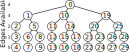
\includegraphics[width=\textwidth]{../app1/fig/dfs}
    \caption{Depth-first search.\label{fig:app1:dfs}}
\end{subfigure}~
\begin{subfigure}[b]{0.48\textwidth}
    \centering
    \includegraphics[width=\textwidth]{../app1/fig/bfs}
    \caption{Breadth-first search.\label{fig:app1:bfs}}
\end{subfigure}
\caption[Two tree traversal strategies.]{Two tree traversal strategies (numbers indicate order the vertices are visited).\label{fig:app1:search}}
\end{figure}

\subsection{Depth-First vs. Breadth-First Search}

% new paragraph
Section~\ref{sec:ch2:treesearch} was titled \textit{Tree Search Algorithm}, but we can be more descriptive of the particular algorithm implementation.
There are two basic methods of tree traversal (the process of visiting each vertex in a directed rooted tree): \glsfirst{DFS} or \glsfirst{BFS} \cite{Skiena2008a, Cormen2009a}.
The primary difference the two methods is the order in which the vertices are explored \cite{Skiena2008a}. 
DFS explores a particular path in the tree to the maximum height possible before backtracking and continuing down an alternative, unexplored path \cite{Cormen2009a}.
This process is visualized in Fig.~\ref{fig:app1:dfs}.
There are both stack-based and recursive implementations of the DFS \cite[pp.~169--172]{Skiena2008a}.
From these definitions, Alg.~\ref{alg:app1:tree} can be classified as a recursive DFS algorithm.
While the current implementation works fairly well, the other tree traversal method, BFS, may be better suited for enumerating the graph structure space of interest.

\begin{figure}[h!]
\centering
\begin{subfigure}[b]{0.5\textwidth}
    \centering
    \includegraphics[scale=0.5]{../app1/fig/isocheck_1}
    \caption{Without level-order isomorphism checking.\label{fig:app1:isocheck_1}}
\end{subfigure}%
\begin{subfigure}[b]{0.5\textwidth}
    \centering
    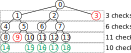
\includegraphics[scale=0.5]{../app1/fig/isocheck_2}
    \caption{With level-order isomorphism checking.\label{fig:app1:isocheck_2}}
\end{subfigure}
\caption[Visualization of the impact of level-order isomorphism checking.]{Visualization of the impact of level-order isomorphism checking during the graph generation process for $(C,R,P) = (\{\xcolor{G},\xcolor{B}\},[1\ 2],[2\ 3])$.\label{fig:app1:isocheck}}
\end{figure}

% new paragraph
A BFS method traverses the tree by visiting each vertex in a particular level first before moving to larger levels through the use of a queue \cite{Skiena2008a, Cormen2009a}.
Levels are defined by sets of vertices with the same height.
This process is visualized in Fig.~\ref{fig:app1:bfs} and note the difference between DFS.
The potential advantage of a BFS implementation would be the ability to include isomorphism checking at each level.
In the current implementation, this is not possible so (potentially) many intermediate graphs that are isomorphic to other intermediate graphs are enumerated.
By identifying isomorphic intermediate graphs, we can remove these vertices (and their subtree) from the tree traversal process.
Thus, there would be a reduction the number of graphs generated while covering the same graph structure space.
However, there is a considerable computational cost associated with checking if a set of graphs is isomorphic (see Sec.~\ref{fig:app1:isocheck}), so there may be cases where the overall computational expense is larger with a BFS implementation with level-order isomorphism checking.

% new paragraph
Consider the example in Fig.~\ref{fig:app1:isocheck} comparing the BFS method with and without level-order isomorphism checking.
The desired set of unique graphs (colored green) is covered by both approaches, but different trees are traversed. 
There is a reduction from a total of 29 generated graphs to 18, but the number of graph comparisons needed only decreases from 31 to 30.
With the overhead associated with calling the isomorphism checking function, level-order isomorphism checking may actually increase computation time.
This is even more likely with the enhancements included because some of the vertices would be removed faster through the enhancements rather than direct isomorphism checking.
It is future work to both implement this enhancement and determine its impact on the overall computational expense.

\subsection{Parallelized Tree Traversal}

We can further leverage our knowledge of the tree structure by parallelizing the traversal process. 
There has been considerable work in parallelizing various graph algorithms \cite{Quinn1984a, Reghbati1978a}.
The enhancement in Sec.~\ref{sec:app1:subcatalogs} for enumerating subcatalogs was a type of parallelized tree traversal, but it is more or less unpredictable in how it partitions the original tree (which was acceptable since it covers the same graph structure space).
There are additional parallel traversal strategies that could be implemented in conjunction with the other enhancements such as the one below.

\begin{figure}[h!]
\centering
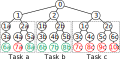
\includegraphics[scale=0.6]{../app1/fig/parallel}
\caption{Parallelization example.\label{fig:app1:parallel}}
\end{figure}

% new paragraph
Consider a tree with $N$ levels.
We can proceed as normal on a single worker using the BFS method up to level $n\leq N$.
At this point, the task of traversing the subtree of each vertex in level $n$ is a parallelizable task (assuming no level-order isomorphism checking).
Level-order isomorphism checking could still be utilized in each of the tasks, but the collected graphs from each of the tasks would still need to be checked for uniqueness.
An example of this approach is shown in Fig.~\ref{fig:app1:parallel} with three tasks and assuming perfect parallelization of the generation task, a reduction from 29 to 13 effective algorithm calls (3 plus the maximum of the tasks).